\documentclass[]{article}
\usepackage{lmodern}
\usepackage{amssymb,amsmath}
\usepackage{ifxetex,ifluatex}
\usepackage{fixltx2e} % provides \textsubscript
\ifnum 0\ifxetex 1\fi\ifluatex 1\fi=0 % if pdftex
  \usepackage[T1]{fontenc}
  \usepackage[utf8]{inputenc}
\else % if luatex or xelatex
  \ifxetex
    \usepackage{mathspec}
  \else
    \usepackage{fontspec}
  \fi
  \defaultfontfeatures{Ligatures=TeX,Scale=MatchLowercase}
\fi
% use upquote if available, for straight quotes in verbatim environments
\IfFileExists{upquote.sty}{\usepackage{upquote}}{}
% use microtype if available
\IfFileExists{microtype.sty}{%
\usepackage{microtype}
\UseMicrotypeSet[protrusion]{basicmath} % disable protrusion for tt fonts
}{}
\usepackage[margin=1in]{geometry}
\usepackage{hyperref}
\hypersetup{unicode=true,
            pdftitle={Reproducible Research: Peer Assessment 1},
            pdfborder={0 0 0},
            breaklinks=true}
\urlstyle{same}  % don't use monospace font for urls
\usepackage{color}
\usepackage{fancyvrb}
\newcommand{\VerbBar}{|}
\newcommand{\VERB}{\Verb[commandchars=\\\{\}]}
\DefineVerbatimEnvironment{Highlighting}{Verbatim}{commandchars=\\\{\}}
% Add ',fontsize=\small' for more characters per line
\usepackage{framed}
\definecolor{shadecolor}{RGB}{248,248,248}
\newenvironment{Shaded}{\begin{snugshade}}{\end{snugshade}}
\newcommand{\KeywordTok}[1]{\textcolor[rgb]{0.13,0.29,0.53}{\textbf{#1}}}
\newcommand{\DataTypeTok}[1]{\textcolor[rgb]{0.13,0.29,0.53}{#1}}
\newcommand{\DecValTok}[1]{\textcolor[rgb]{0.00,0.00,0.81}{#1}}
\newcommand{\BaseNTok}[1]{\textcolor[rgb]{0.00,0.00,0.81}{#1}}
\newcommand{\FloatTok}[1]{\textcolor[rgb]{0.00,0.00,0.81}{#1}}
\newcommand{\ConstantTok}[1]{\textcolor[rgb]{0.00,0.00,0.00}{#1}}
\newcommand{\CharTok}[1]{\textcolor[rgb]{0.31,0.60,0.02}{#1}}
\newcommand{\SpecialCharTok}[1]{\textcolor[rgb]{0.00,0.00,0.00}{#1}}
\newcommand{\StringTok}[1]{\textcolor[rgb]{0.31,0.60,0.02}{#1}}
\newcommand{\VerbatimStringTok}[1]{\textcolor[rgb]{0.31,0.60,0.02}{#1}}
\newcommand{\SpecialStringTok}[1]{\textcolor[rgb]{0.31,0.60,0.02}{#1}}
\newcommand{\ImportTok}[1]{#1}
\newcommand{\CommentTok}[1]{\textcolor[rgb]{0.56,0.35,0.01}{\textit{#1}}}
\newcommand{\DocumentationTok}[1]{\textcolor[rgb]{0.56,0.35,0.01}{\textbf{\textit{#1}}}}
\newcommand{\AnnotationTok}[1]{\textcolor[rgb]{0.56,0.35,0.01}{\textbf{\textit{#1}}}}
\newcommand{\CommentVarTok}[1]{\textcolor[rgb]{0.56,0.35,0.01}{\textbf{\textit{#1}}}}
\newcommand{\OtherTok}[1]{\textcolor[rgb]{0.56,0.35,0.01}{#1}}
\newcommand{\FunctionTok}[1]{\textcolor[rgb]{0.00,0.00,0.00}{#1}}
\newcommand{\VariableTok}[1]{\textcolor[rgb]{0.00,0.00,0.00}{#1}}
\newcommand{\ControlFlowTok}[1]{\textcolor[rgb]{0.13,0.29,0.53}{\textbf{#1}}}
\newcommand{\OperatorTok}[1]{\textcolor[rgb]{0.81,0.36,0.00}{\textbf{#1}}}
\newcommand{\BuiltInTok}[1]{#1}
\newcommand{\ExtensionTok}[1]{#1}
\newcommand{\PreprocessorTok}[1]{\textcolor[rgb]{0.56,0.35,0.01}{\textit{#1}}}
\newcommand{\AttributeTok}[1]{\textcolor[rgb]{0.77,0.63,0.00}{#1}}
\newcommand{\RegionMarkerTok}[1]{#1}
\newcommand{\InformationTok}[1]{\textcolor[rgb]{0.56,0.35,0.01}{\textbf{\textit{#1}}}}
\newcommand{\WarningTok}[1]{\textcolor[rgb]{0.56,0.35,0.01}{\textbf{\textit{#1}}}}
\newcommand{\AlertTok}[1]{\textcolor[rgb]{0.94,0.16,0.16}{#1}}
\newcommand{\ErrorTok}[1]{\textcolor[rgb]{0.64,0.00,0.00}{\textbf{#1}}}
\newcommand{\NormalTok}[1]{#1}
\usepackage{graphicx,grffile}
\makeatletter
\def\maxwidth{\ifdim\Gin@nat@width>\linewidth\linewidth\else\Gin@nat@width\fi}
\def\maxheight{\ifdim\Gin@nat@height>\textheight\textheight\else\Gin@nat@height\fi}
\makeatother
% Scale images if necessary, so that they will not overflow the page
% margins by default, and it is still possible to overwrite the defaults
% using explicit options in \includegraphics[width, height, ...]{}
\setkeys{Gin}{width=\maxwidth,height=\maxheight,keepaspectratio}
\IfFileExists{parskip.sty}{%
\usepackage{parskip}
}{% else
\setlength{\parindent}{0pt}
\setlength{\parskip}{6pt plus 2pt minus 1pt}
}
\setlength{\emergencystretch}{3em}  % prevent overfull lines
\providecommand{\tightlist}{%
  \setlength{\itemsep}{0pt}\setlength{\parskip}{0pt}}
\setcounter{secnumdepth}{0}
% Redefines (sub)paragraphs to behave more like sections
\ifx\paragraph\undefined\else
\let\oldparagraph\paragraph
\renewcommand{\paragraph}[1]{\oldparagraph{#1}\mbox{}}
\fi
\ifx\subparagraph\undefined\else
\let\oldsubparagraph\subparagraph
\renewcommand{\subparagraph}[1]{\oldsubparagraph{#1}\mbox{}}
\fi

%%% Use protect on footnotes to avoid problems with footnotes in titles
\let\rmarkdownfootnote\footnote%
\def\footnote{\protect\rmarkdownfootnote}

%%% Change title format to be more compact
\usepackage{titling}

% Create subtitle command for use in maketitle
\newcommand{\subtitle}[1]{
  \posttitle{
    \begin{center}\large#1\end{center}
    }
}

\setlength{\droptitle}{-2em}
  \title{Reproducible Research: Peer Assessment 1}
  \pretitle{\vspace{\droptitle}\centering\huge}
  \posttitle{\par}
  \author{}
  \preauthor{}\postauthor{}
  \date{}
  \predate{}\postdate{}


\begin{document}
\maketitle

\subsection{Author : Nima Arvin}\label{author-nima-arvin}

\subsection{setting the global options to show the code and results for
all code
chunks}\label{setting-the-global-options-to-show-the-code-and-results-for-all-code-chunks}

\begin{Shaded}
\begin{Highlighting}[]
\NormalTok{knitr}\OperatorTok{::}\NormalTok{opts_chunk}\OperatorTok{$}\KeywordTok{set}\NormalTok{(}\DataTypeTok{echo =} \OtherTok{TRUE}\NormalTok{)}
\end{Highlighting}
\end{Shaded}

\subsection{Code for reading in the dataset and/or processing the
data}\label{code-for-reading-in-the-dataset-andor-processing-the-data}

\begin{Shaded}
\begin{Highlighting}[]
\KeywordTok{library}\NormalTok{(knitr)}
\KeywordTok{library}\NormalTok{(lubridate)}
\end{Highlighting}
\end{Shaded}

\begin{verbatim}
## 
## Attaching package: 'lubridate'
\end{verbatim}

\begin{verbatim}
## The following object is masked from 'package:base':
## 
##     date
\end{verbatim}

\begin{Shaded}
\begin{Highlighting}[]
\NormalTok{wd <-}\StringTok{ }\KeywordTok{getwd}\NormalTok{()}
\NormalTok{zipfile <-}\KeywordTok{download.file}\NormalTok{(}\StringTok{"https://d396qusza40orc.cloudfront.net/repdata%2Fdata%2Factivity.zip"}\NormalTok{,}\DataTypeTok{destfile=}\KeywordTok{paste0}\NormalTok{(wd,}\StringTok{"/file.zip"}\NormalTok{)) }
\KeywordTok{unzip}\NormalTok{(}\KeywordTok{paste0}\NormalTok{(wd,}\StringTok{"/file.zip"}\NormalTok{))}
\NormalTok{maindata <-}\StringTok{ }\KeywordTok{read.csv}\NormalTok{(}\KeywordTok{paste0}\NormalTok{(wd,}\StringTok{"/activity.csv"}\NormalTok{), }\DataTypeTok{header =} \OtherTok{TRUE}\NormalTok{)}
\NormalTok{maindata}\OperatorTok{$}\NormalTok{date <-}\StringTok{ }\KeywordTok{ymd}\NormalTok{(maindata}\OperatorTok{$}\NormalTok{date)}
\KeywordTok{summary}\NormalTok{(maindata)}
\end{Highlighting}
\end{Shaded}

\begin{verbatim}
##      steps             date               interval     
##  Min.   :  0.00   Min.   :2012-10-01   Min.   :   0.0  
##  1st Qu.:  0.00   1st Qu.:2012-10-16   1st Qu.: 588.8  
##  Median :  0.00   Median :2012-10-31   Median :1177.5  
##  Mean   : 37.38   Mean   :2012-10-31   Mean   :1177.5  
##  3rd Qu.: 12.00   3rd Qu.:2012-11-15   3rd Qu.:1766.2  
##  Max.   :806.00   Max.   :2012-11-30   Max.   :2355.0  
##  NA's   :2304
\end{verbatim}

\begin{Shaded}
\begin{Highlighting}[]
\KeywordTok{str}\NormalTok{(maindata)}
\end{Highlighting}
\end{Shaded}

\begin{verbatim}
## 'data.frame':    17568 obs. of  3 variables:
##  $ steps   : int  NA NA NA NA NA NA NA NA NA NA ...
##  $ date    : Date, format: "2012-10-01" "2012-10-01" ...
##  $ interval: int  0 5 10 15 20 25 30 35 40 45 ...
\end{verbatim}

\subsection{Daily Activity Pattern}\label{daily-activity-pattern}

\subsubsection{What is mean total number of steps taken per
day?}\label{what-is-mean-total-number-of-steps-taken-per-day}

\begin{Shaded}
\begin{Highlighting}[]
\KeywordTok{library}\NormalTok{(dplyr)}
\end{Highlighting}
\end{Shaded}

\begin{verbatim}
## 
## Attaching package: 'dplyr'
\end{verbatim}

\begin{verbatim}
## The following objects are masked from 'package:stats':
## 
##     filter, lag
\end{verbatim}

\begin{verbatim}
## The following objects are masked from 'package:base':
## 
##     intersect, setdiff, setequal, union
\end{verbatim}

\begin{Shaded}
\begin{Highlighting}[]
\NormalTok{gdata <-}\StringTok{ }\KeywordTok{group_by}\NormalTok{(maindata, date)}
\NormalTok{dailymeans<-}\StringTok{ }\KeywordTok{summarise}\NormalTok{(gdata, }\DataTypeTok{mean=}\KeywordTok{mean}\NormalTok{(steps, }\DataTypeTok{na.rm =} \OtherTok{TRUE}\NormalTok{))}
\NormalTok{dailymeans}
\end{Highlighting}
\end{Shaded}

\begin{verbatim}
## # A tibble: 61 x 2
##    date          mean
##    <date>       <dbl>
##  1 2012-10-01 NaN    
##  2 2012-10-02   0.438
##  3 2012-10-03  39.4  
##  4 2012-10-04  42.1  
##  5 2012-10-05  46.2  
##  6 2012-10-06  53.5  
##  7 2012-10-07  38.2  
##  8 2012-10-08 NaN    
##  9 2012-10-09  44.5  
## 10 2012-10-10  34.4  
## # ... with 51 more rows
\end{verbatim}

\subsubsection{Median number of steps taken each
day}\label{median-number-of-steps-taken-each-day}

\begin{Shaded}
\begin{Highlighting}[]
\NormalTok{dailymedians<-}\StringTok{ }\KeywordTok{summarise}\NormalTok{(gdata, }\DataTypeTok{mean=}\KeywordTok{median}\NormalTok{(steps, }\DataTypeTok{na.rm =} \OtherTok{TRUE}\NormalTok{))}
\NormalTok{dailymedians}
\end{Highlighting}
\end{Shaded}

\begin{verbatim}
## # A tibble: 61 x 2
##    date        mean
##    <date>     <dbl>
##  1 2012-10-01    NA
##  2 2012-10-02     0
##  3 2012-10-03     0
##  4 2012-10-04     0
##  5 2012-10-05     0
##  6 2012-10-06     0
##  7 2012-10-07     0
##  8 2012-10-08    NA
##  9 2012-10-09     0
## 10 2012-10-10     0
## # ... with 51 more rows
\end{verbatim}

\subsubsection{Total number of steps taken per
day}\label{total-number-of-steps-taken-per-day}

\begin{Shaded}
\begin{Highlighting}[]
\NormalTok{dailytotals <-}\StringTok{ }\KeywordTok{summarise}\NormalTok{(gdata, }\DataTypeTok{totals=}\KeywordTok{sum}\NormalTok{(steps, }\DataTypeTok{na.rm =} \OtherTok{TRUE}\NormalTok{))}
\NormalTok{dailytotals}
\end{Highlighting}
\end{Shaded}

\begin{verbatim}
## # A tibble: 61 x 2
##    date       totals
##    <date>      <int>
##  1 2012-10-01      0
##  2 2012-10-02    126
##  3 2012-10-03  11352
##  4 2012-10-04  12116
##  5 2012-10-05  13294
##  6 2012-10-06  15420
##  7 2012-10-07  11015
##  8 2012-10-08      0
##  9 2012-10-09  12811
## 10 2012-10-10   9900
## # ... with 51 more rows
\end{verbatim}

\subsubsection{Histogram of the total number of steps taken each
day}\label{histogram-of-the-total-number-of-steps-taken-each-day}

\begin{Shaded}
\begin{Highlighting}[]
\KeywordTok{with}\NormalTok{(dailytotals,}\KeywordTok{hist}\NormalTok{(totals, }\DataTypeTok{col =} \StringTok{"green"}\NormalTok{))}
\end{Highlighting}
\end{Shaded}

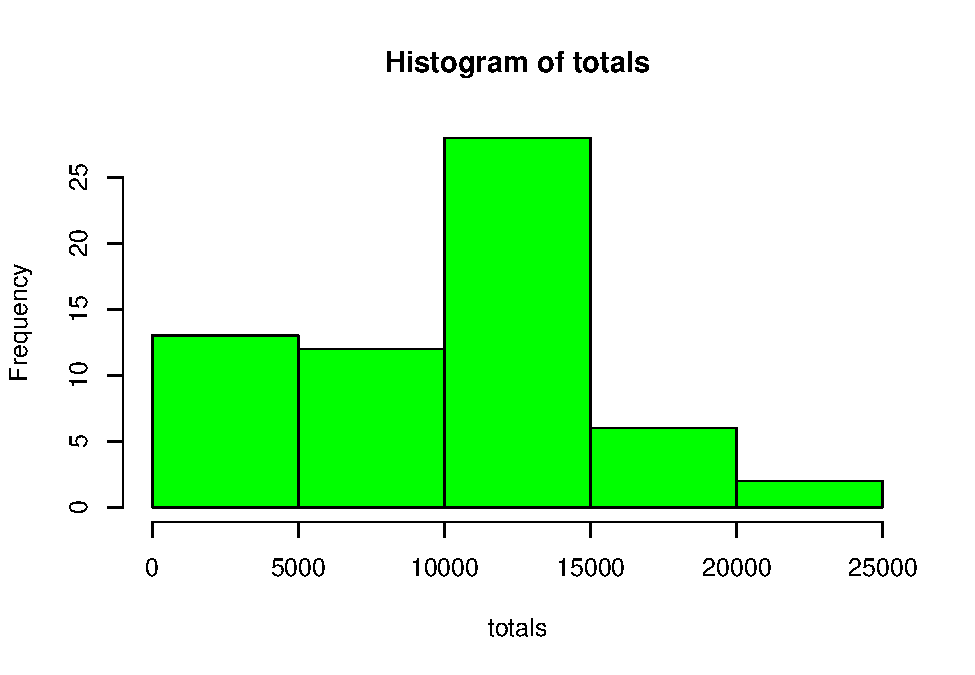
\includegraphics{PA1_template_files/figure-latex/unnamed-chunk-5-1.pdf}

\subsubsection{Mean and Median of the total number of steps taken per
day}\label{mean-and-median-of-the-total-number-of-steps-taken-per-day}

\begin{Shaded}
\begin{Highlighting}[]
\NormalTok{### Mean of total number of steps per day}
\KeywordTok{mean}\NormalTok{(dailytotals}\OperatorTok{$}\NormalTok{totals)}
\end{Highlighting}
\end{Shaded}

\begin{verbatim}
## [1] 9354.23
\end{verbatim}

\begin{Shaded}
\begin{Highlighting}[]
\NormalTok{### Median of total number of steps per day}
\KeywordTok{median}\NormalTok{(dailytotals}\OperatorTok{$}\NormalTok{totals)}
\end{Highlighting}
\end{Shaded}

\begin{verbatim}
## [1] 10395
\end{verbatim}

\subsubsection{Time series plot of the 5 minutes
interval}\label{time-series-plot-of-the-5-minutes-interval}

\begin{Shaded}
\begin{Highlighting}[]
\KeywordTok{library}\NormalTok{(dplyr)}
\KeywordTok{library}\NormalTok{(ggplot2)}
\NormalTok{gidata <-}\StringTok{ }\KeywordTok{group_by}\NormalTok{(maindata, interval)}
\NormalTok{intervalmeans <-}\StringTok{ }\KeywordTok{summarize}\NormalTok{(gidata, }\DataTypeTok{intmeans=}\KeywordTok{mean}\NormalTok{(steps, }\DataTypeTok{na.rm =} \OtherTok{TRUE}\NormalTok{))}
\NormalTok{intervalmeans}
\end{Highlighting}
\end{Shaded}

\begin{verbatim}
## # A tibble: 288 x 2
##    interval intmeans
##       <int>    <dbl>
##  1        0   1.72  
##  2        5   0.340 
##  3       10   0.132 
##  4       15   0.151 
##  5       20   0.0755
##  6       25   2.09  
##  7       30   0.528 
##  8       35   0.868 
##  9       40   0     
## 10       45   1.47  
## # ... with 278 more rows
\end{verbatim}

\begin{Shaded}
\begin{Highlighting}[]
\NormalTok{g2 <-}\StringTok{ }\KeywordTok{ggplot}\NormalTok{(intervalmeans, }\KeywordTok{aes}\NormalTok{(interval, intmeans, }\DataTypeTok{group=}\DecValTok{1}\NormalTok{))}
\NormalTok{g2}\OperatorTok{+}\KeywordTok{geom_point}\NormalTok{(}\DataTypeTok{col=}\StringTok{"black"}\NormalTok{, }\DataTypeTok{size=}\DecValTok{1}\NormalTok{)}\OperatorTok{+}\KeywordTok{geom_line}\NormalTok{(}\DataTypeTok{col=}\StringTok{"red"}\NormalTok{)}\OperatorTok{+}\KeywordTok{labs}\NormalTok{(}\DataTypeTok{title=}\StringTok{"Mean of number of steps per intervals"}\NormalTok{, }\DataTypeTok{x=}\StringTok{"Intervals observed"}\NormalTok{, }\DataTypeTok{y=}\StringTok{"Mean of number of steps"}\NormalTok{)}
\end{Highlighting}
\end{Shaded}

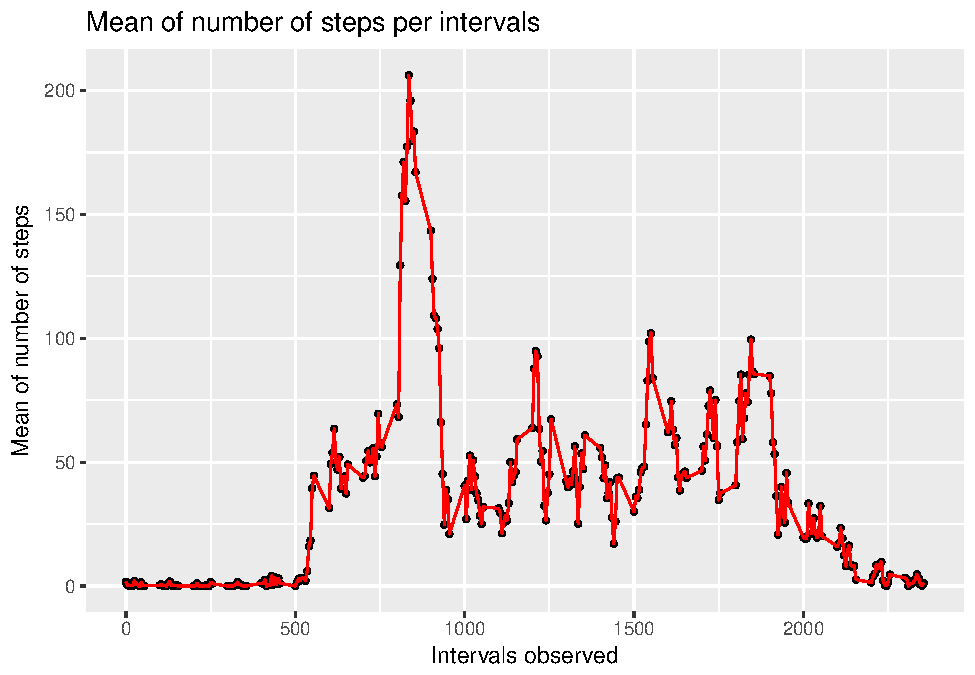
\includegraphics{PA1_template_files/figure-latex/unnamed-chunk-7-1.pdf}

\subsubsection{Which 5-minute interval, on average across all the days
in the dataset, contains the maximum number of
steps?}\label{which-5-minute-interval-on-average-across-all-the-days-in-the-dataset-contains-the-maximum-number-of-steps}

\begin{Shaded}
\begin{Highlighting}[]
\NormalTok{intervalmeans[intervalmeans[,}\DecValTok{2}\NormalTok{]}\OperatorTok{==}\KeywordTok{max}\NormalTok{(intervalmeans[,}\DecValTok{2}\NormalTok{]),]}
\end{Highlighting}
\end{Shaded}

\begin{verbatim}
## # A tibble: 1 x 2
##   interval intmeans
##      <int>    <dbl>
## 1      835     206.
\end{verbatim}

\subsubsection{Time series plot of the average number of steps
taken}\label{time-series-plot-of-the-average-number-of-steps-taken}

\begin{Shaded}
\begin{Highlighting}[]
\NormalTok{g <-}\StringTok{ }\KeywordTok{ggplot}\NormalTok{(dailymeans, }\KeywordTok{aes}\NormalTok{(date,mean, }\DataTypeTok{group=}\DecValTok{1}\NormalTok{))}
\NormalTok{g }\OperatorTok{+}\StringTok{ }\KeywordTok{geom_point}\NormalTok{(}\DataTypeTok{col=}\StringTok{"red"}\NormalTok{)}\OperatorTok{+}\StringTok{ }\KeywordTok{geom_line}\NormalTok{()}\OperatorTok{+}\KeywordTok{geom_smooth}\NormalTok{(}\DataTypeTok{method =} \StringTok{"glm"}\NormalTok{, }\DataTypeTok{na.rm =} \OtherTok{TRUE}\NormalTok{)}\OperatorTok{+}\StringTok{ }\KeywordTok{theme}\NormalTok{(}\DataTypeTok{axis.text.x =} \KeywordTok{element_text}\NormalTok{(}\DataTypeTok{angle =} \DecValTok{90}\NormalTok{, }\DataTypeTok{hjust =} \DecValTok{1}\NormalTok{))}\OperatorTok{+}\KeywordTok{labs}\NormalTok{(}\DataTypeTok{title=}\StringTok{"Average Steps Per Day"}\NormalTok{,}\DataTypeTok{x=}\StringTok{"Observation Date"}\NormalTok{,}\DataTypeTok{y=}\StringTok{"Mean of number of steps"}\NormalTok{ )}
\end{Highlighting}
\end{Shaded}

\begin{verbatim}
## Warning: Removed 8 rows containing missing values (geom_point).
\end{verbatim}

\begin{verbatim}
## Warning: Removed 2 rows containing missing values (geom_path).
\end{verbatim}

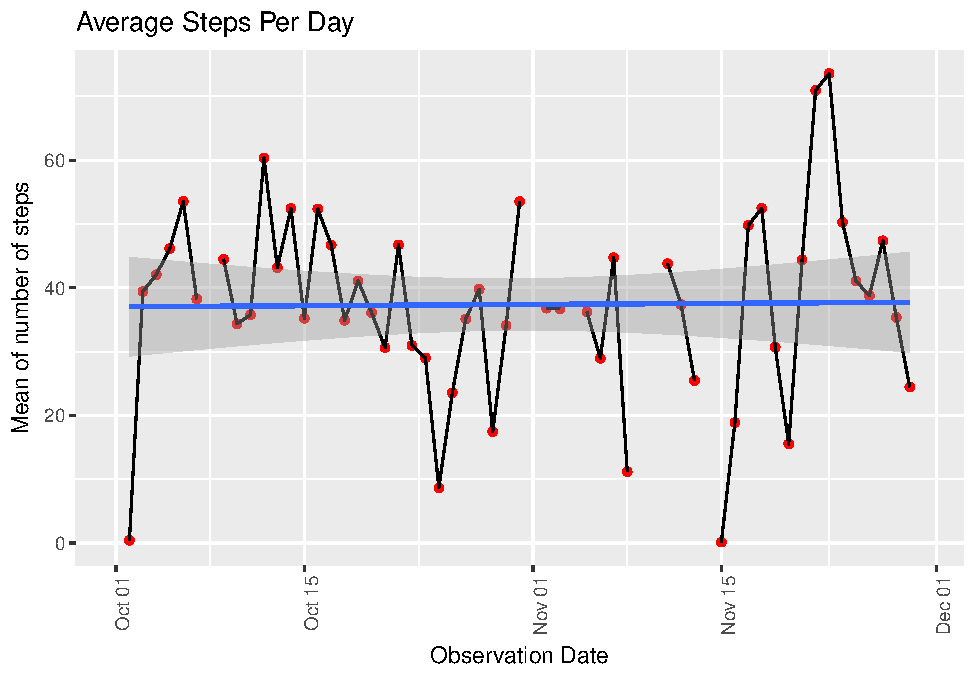
\includegraphics{PA1_template_files/figure-latex/unnamed-chunk-9-1.pdf}

\subsubsection{Are there differences in activity patterns between
weekdays and
weekends?}\label{are-there-differences-in-activity-patterns-between-weekdays-and-weekends}

\begin{Shaded}
\begin{Highlighting}[]
\KeywordTok{library}\NormalTok{(lubridate)}
\end{Highlighting}
\end{Shaded}

\begin{verbatim}
## 
## Attaching package: 'lubridate'
\end{verbatim}

\begin{verbatim}
## The following object is masked from 'package:base':
## 
##     date
\end{verbatim}

\begin{Shaded}
\begin{Highlighting}[]
\NormalTok{dailytotals}\OperatorTok{$}\NormalTok{weekday <-}\StringTok{ }\KeywordTok{wday}\NormalTok{(dailytotals}\OperatorTok{$}\NormalTok{date, }\DataTypeTok{label =} \OtherTok{TRUE}\NormalTok{)}
\NormalTok{wdg <-}\StringTok{ }\KeywordTok{group_by}\NormalTok{(dailytotals, weekday)}
\NormalTok{weekdayavg <-}\StringTok{ }\KeywordTok{summarize}\NormalTok{(wdg, }\DataTypeTok{WeekdayAverage=}\KeywordTok{mean}\NormalTok{(totals, }\DataTypeTok{na.rm =} \OtherTok{TRUE}\NormalTok{))}
\NormalTok{g3 <-}\StringTok{ }\KeywordTok{ggplot}\NormalTok{(weekdayavg, }\KeywordTok{aes}\NormalTok{(weekday,WeekdayAverage, }\DataTypeTok{group=}\DecValTok{1}\NormalTok{))}
\NormalTok{g3}\OperatorTok{+}\KeywordTok{geom_point}\NormalTok{(}\DataTypeTok{col=}\StringTok{"black"}\NormalTok{, }\DataTypeTok{size=}\DecValTok{2}\NormalTok{)}\OperatorTok{+}\KeywordTok{geom_line}\NormalTok{(}\DataTypeTok{col=}\StringTok{"red"}\NormalTok{)}
\end{Highlighting}
\end{Shaded}

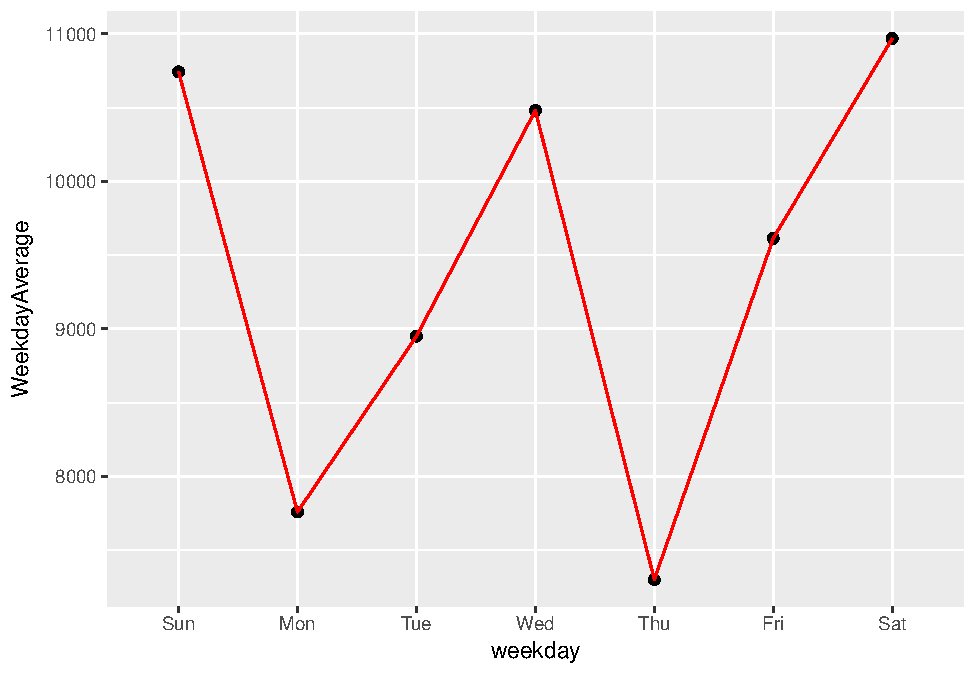
\includegraphics{PA1_template_files/figure-latex/unnamed-chunk-10-1.pdf}

\subsubsection{How did the weekdays trend looked like over time
?}\label{how-did-the-weekdays-trend-looked-like-over-time}

\begin{Shaded}
\begin{Highlighting}[]
\NormalTok{dailytotals}\OperatorTok{$}\NormalTok{weekday <-}\StringTok{ }\KeywordTok{wday}\NormalTok{(dailytotals}\OperatorTok{$}\NormalTok{date, }\DataTypeTok{label =} \OtherTok{TRUE}\NormalTok{)}
\NormalTok{g1 <-}\StringTok{ }\KeywordTok{ggplot}\NormalTok{(dailytotals, }\KeywordTok{aes}\NormalTok{(date, totals, }\DataTypeTok{group=}\NormalTok{weekday))}
\NormalTok{g1}\OperatorTok{+}\KeywordTok{geom_point}\NormalTok{(}\DataTypeTok{size=}\DecValTok{1}\NormalTok{, }\DataTypeTok{col=}\StringTok{"black"}\NormalTok{)}\OperatorTok{+}\KeywordTok{geom_line}\NormalTok{(}\DataTypeTok{col=}\StringTok{"red"}\NormalTok{)}\OperatorTok{+}\KeywordTok{facet_grid}\NormalTok{(.}\OperatorTok{~}\NormalTok{weekday)}\OperatorTok{+}\KeywordTok{theme}\NormalTok{(}\DataTypeTok{axis.text.x =} \KeywordTok{element_text}\NormalTok{(}\DataTypeTok{angle =} \DecValTok{90}\NormalTok{, }\DataTypeTok{hjust =} \DecValTok{1}\NormalTok{))}\OperatorTok{+}\KeywordTok{geom_smooth}\NormalTok{(}\DataTypeTok{method =} \StringTok{"lm"}\NormalTok{)}
\end{Highlighting}
\end{Shaded}

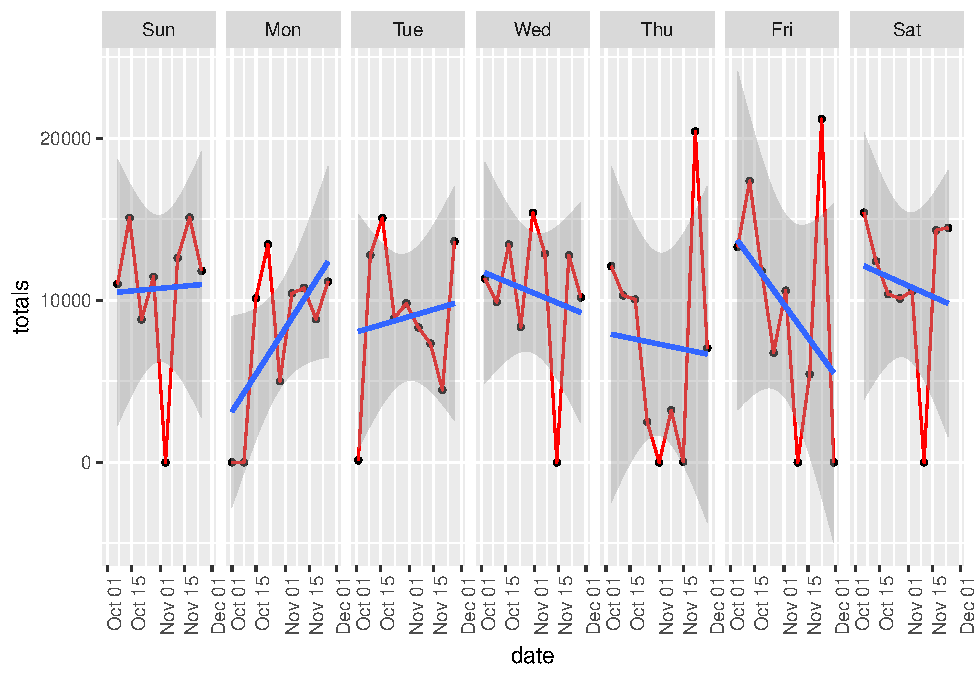
\includegraphics{PA1_template_files/figure-latex/unnamed-chunk-11-1.pdf}

\subsubsection{Panel plot comparing the average number of steps taken
per 5-minute interval across weekdays and
weekends}\label{panel-plot-comparing-the-average-number-of-steps-taken-per-5-minute-interval-across-weekdays-and-weekends}

\begin{Shaded}
\begin{Highlighting}[]
\NormalTok{day <-}\StringTok{ }\KeywordTok{weekdays}\NormalTok{(maindata}\OperatorTok{$}\NormalTok{date)}
\NormalTok{daylevel <-}\StringTok{ }\KeywordTok{vector}\NormalTok{()}
\ControlFlowTok{for}\NormalTok{ (i }\ControlFlowTok{in} \DecValTok{1}\OperatorTok{:}\KeywordTok{nrow}\NormalTok{(maindata)) \{}
    \ControlFlowTok{if}\NormalTok{ (day[i] }\OperatorTok{==}\StringTok{ "Saturday"}\NormalTok{) \{}
\NormalTok{        daylevel[i] <-}\StringTok{ "Weekend"}
\NormalTok{    \} }\ControlFlowTok{else} \ControlFlowTok{if}\NormalTok{ (day[i] }\OperatorTok{==}\StringTok{ "Sunday"}\NormalTok{) \{}
\NormalTok{        daylevel[i] <-}\StringTok{ "Weekend"}
\NormalTok{    \} }\ControlFlowTok{else}\NormalTok{ \{}
\NormalTok{        daylevel[i] <-}\StringTok{ "Weekday"}
\NormalTok{    \}}
\NormalTok{\}}
\NormalTok{maindata}\OperatorTok{$}\NormalTok{daylevel <-}\StringTok{ }\NormalTok{daylevel}
\NormalTok{maindata}\OperatorTok{$}\NormalTok{daylevel <-}\StringTok{ }\KeywordTok{factor}\NormalTok{(maindata}\OperatorTok{$}\NormalTok{daylevel)}

\NormalTok{gint <-}\StringTok{ }\KeywordTok{group_by}\NormalTok{(maindata, daylevel, interval)}
\NormalTok{aint <-}\StringTok{ }\KeywordTok{summarize}\NormalTok{(gint,}\DataTypeTok{ave=}\KeywordTok{mean}\NormalTok{(steps, }\DataTypeTok{na.rm =} \OtherTok{TRUE}\NormalTok{) )}


\NormalTok{g4 <-}\StringTok{ }\KeywordTok{ggplot}\NormalTok{(aint, }\KeywordTok{aes}\NormalTok{(interval, ave, }\DataTypeTok{group=}\DecValTok{1}\NormalTok{))}
\NormalTok{g4}\OperatorTok{+}\KeywordTok{geom_point}\NormalTok{(}\DataTypeTok{size=}\DecValTok{1}\NormalTok{, }\DataTypeTok{col=}\StringTok{"red"}\NormalTok{)}\OperatorTok{+}\StringTok{ }\KeywordTok{geom_line}\NormalTok{(}\DataTypeTok{col=}\StringTok{"black"}\NormalTok{)}\OperatorTok{+}\KeywordTok{facet_grid}\NormalTok{(daylevel}\OperatorTok{~}\NormalTok{.)}
\end{Highlighting}
\end{Shaded}

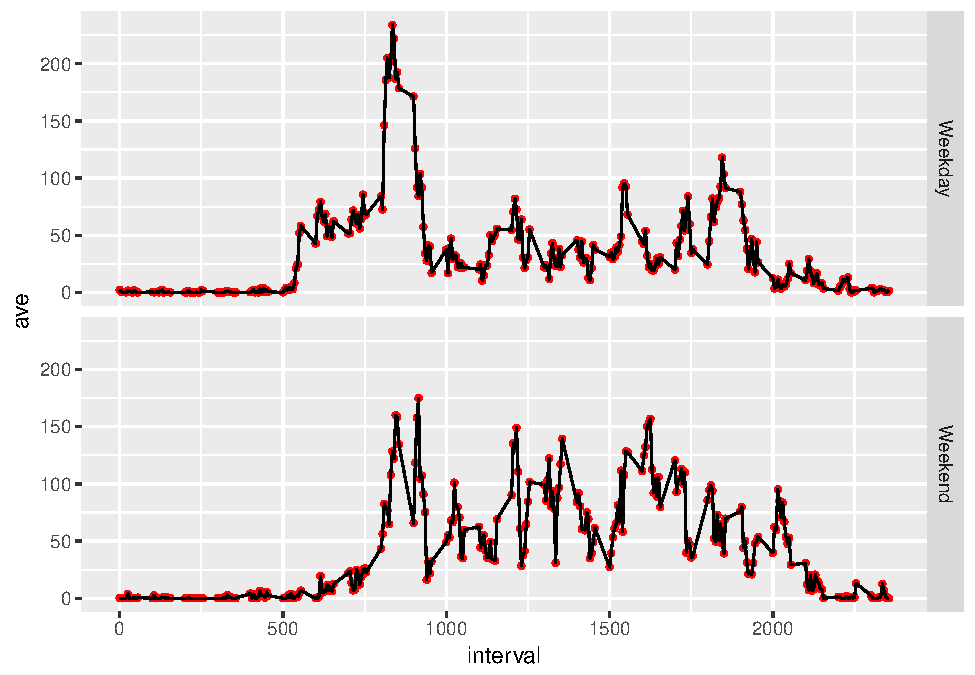
\includegraphics{PA1_template_files/figure-latex/unnamed-chunk-12-1.pdf}

\subsection{Imputing missing values}\label{imputing-missing-values}

\subsubsection{Calculate and report the total number of lines with
missing values in the
dataset}\label{calculate-and-report-the-total-number-of-lines-with-missing-values-in-the-dataset}

\begin{Shaded}
\begin{Highlighting}[]
\KeywordTok{sum}\NormalTok{(}\KeywordTok{is.na}\NormalTok{(maindata))}
\end{Highlighting}
\end{Shaded}

\begin{verbatim}
## [1] 2304
\end{verbatim}

\subsubsection{Get a report of the columns that have missing
values}\label{get-a-report-of-the-columns-that-have-missing-values}

\begin{Shaded}
\begin{Highlighting}[]
\KeywordTok{summary}\NormalTok{(}\KeywordTok{is.na}\NormalTok{(maindata))}
\end{Highlighting}
\end{Shaded}

\begin{verbatim}
##    steps            date          interval        daylevel      
##  Mode :logical   Mode :logical   Mode :logical   Mode :logical  
##  FALSE:15264     FALSE:17568     FALSE:17568     FALSE:17568    
##  TRUE :2304
\end{verbatim}

\subsubsection{Code to describe and show a strategy for imputing missing
data}\label{code-to-describe-and-show-a-strategy-for-imputing-missing-data}

\begin{enumerate}
\def\labelenumi{\arabic{enumi}.}
\tightlist
\item
  The strategy will be to substitude the missing value with the mean of
  the number of steps for that interval
\end{enumerate}

\begin{Shaded}
\begin{Highlighting}[]
\NormalTok{z <-}\StringTok{ }\KeywordTok{aggregate}\NormalTok{(steps}\OperatorTok{~}\StringTok{ }\NormalTok{interval, }\DataTypeTok{data =}\NormalTok{ maindata,mean)}
\ControlFlowTok{for}\NormalTok{ (i }\ControlFlowTok{in} \DecValTok{1}\OperatorTok{:}\KeywordTok{nrow}\NormalTok{(maindata)) \{}
    \ControlFlowTok{if}\NormalTok{ (}\KeywordTok{is.na}\NormalTok{(maindata}\OperatorTok{$}\NormalTok{steps[i])) \{}
\NormalTok{        maindata}\OperatorTok{$}\NormalTok{steps[i] <-}\StringTok{ }\NormalTok{z[z[,}\DecValTok{1}\NormalTok{]}\OperatorTok{==}\NormalTok{maindata}\OperatorTok{$}\NormalTok{interval[i],}\DecValTok{2}\NormalTok{]}
\NormalTok{    \}}
\NormalTok{\}}
\NormalTok{maindata.no.missing <-}\StringTok{ }\NormalTok{maindata}
\KeywordTok{summary}\NormalTok{(}\KeywordTok{is.na}\NormalTok{(maindata.no.missing))}
\end{Highlighting}
\end{Shaded}

\begin{verbatim}
##    steps            date          interval        daylevel      
##  Mode :logical   Mode :logical   Mode :logical   Mode :logical  
##  FALSE:17568     FALSE:17568     FALSE:17568     FALSE:17568
\end{verbatim}

\subsubsection{Histogram of the total number of steps taken each day
after missing values are
imputed}\label{histogram-of-the-total-number-of-steps-taken-each-day-after-missing-values-are-imputed}

\begin{Shaded}
\begin{Highlighting}[]
\NormalTok{ggroup <-}\StringTok{ }\KeywordTok{summarise}\NormalTok{(}\KeywordTok{group_by}\NormalTok{(maindata.no.missing, date),}\DataTypeTok{sum=}\KeywordTok{sum}\NormalTok{(steps, }\DataTypeTok{na.rm =} \OtherTok{TRUE}\NormalTok{))}
\KeywordTok{with}\NormalTok{(ggroup, }\KeywordTok{hist}\NormalTok{(sum, }\DataTypeTok{col =} \StringTok{"red"}\NormalTok{))}
\end{Highlighting}
\end{Shaded}

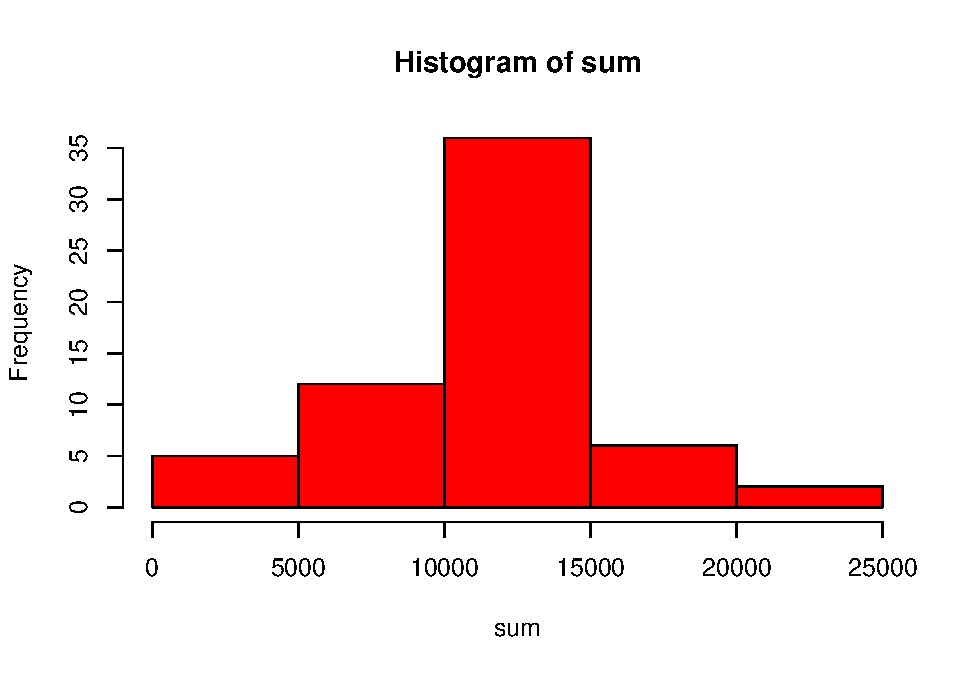
\includegraphics{PA1_template_files/figure-latex/unnamed-chunk-16-1.pdf}


\end{document}
